\chapter{Visualisation}
This report outlines the steps taken to develop a handwritten multi-digit classifier using multiple machine learning techniques. A random sample of images and labels from the provided dataset displays the challenges of implementing such classifier. The red markings in \autoref{fig:sampleImage} highlight a few poorly written digits and additional noise.

\begin{figure}[h]
    \centering
    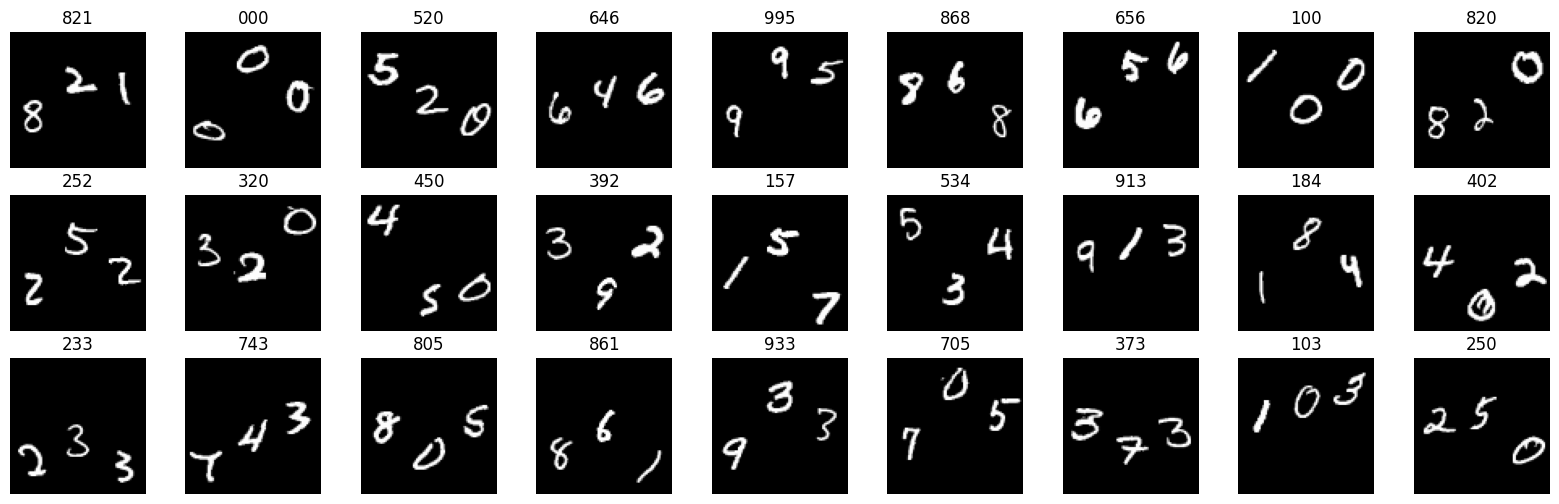
\includegraphics[width=\textwidth, height=\textheight,keepaspectratio]{task1/digitSample}
    \caption[Random sample of images and labels]
    {Random sample of images and labels}
    \label{fig:sampleImage}
\end{figure}

There are 640, 200 and 160 classes present in the train, test, and validation sets, all classes contain 100 images.  The images are greyscale. The distribution graphs display when a class is present in a set. The red lines indicate which classes are present in the test or validation sets but not present in the train set. Unfortunately, this shows that all classes in the test and validation set are not in the train set. Using the dataset as it is, with single labels, learning from the training set cannot transfer into the validation and test sets.

\begin{figure}[h]
    \centering
    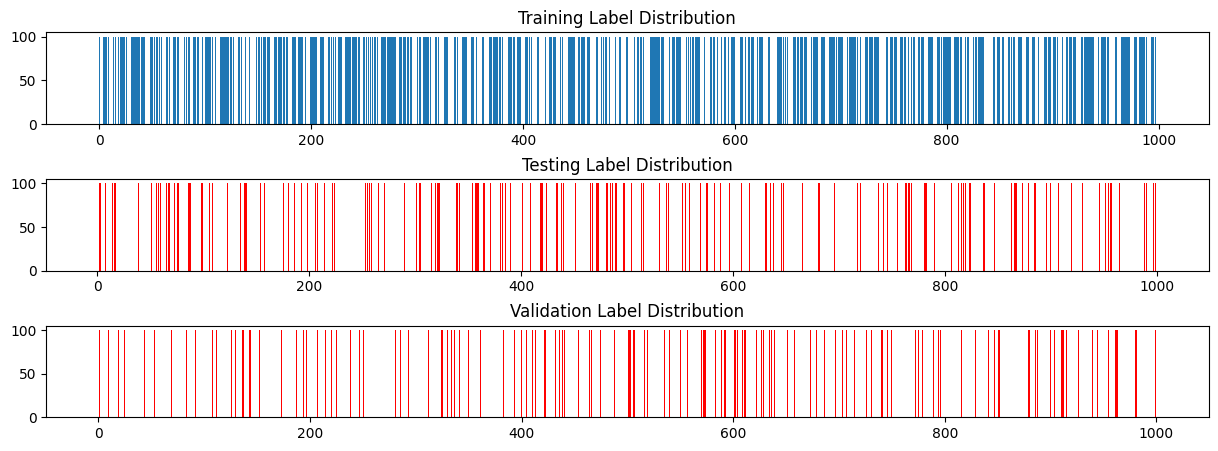
\includegraphics[width=\textwidth, height=\textheight,keepaspectratio]{task1/classDistribution}
    \caption[Distribution graph for datasets]
    {Distribution graph for test/train/validation datasets}
    \label{fig:classDistribution}
\end{figure}

Instead, this should be treated as a multi-label classification problem, with each label representing a digit. For example, the image containing 123 does not contain a single label of “123” but rather three labels of “1”, “2”, and “3”.

When treated as a multi-label classification problem, analysis of the placement of the digits can take place. The heatmap displays the proportion of the digits at a specific location within the images. Ideally the distribution is 0.1 per digit (10\%) at each location. Train is the most evenly distributed set in \autoref{fig:heatmap}, likely due to its size.  This is most optimal as during training the model shall receive an even exposure of all digits.

\begin{figure}[h]
    \centering
    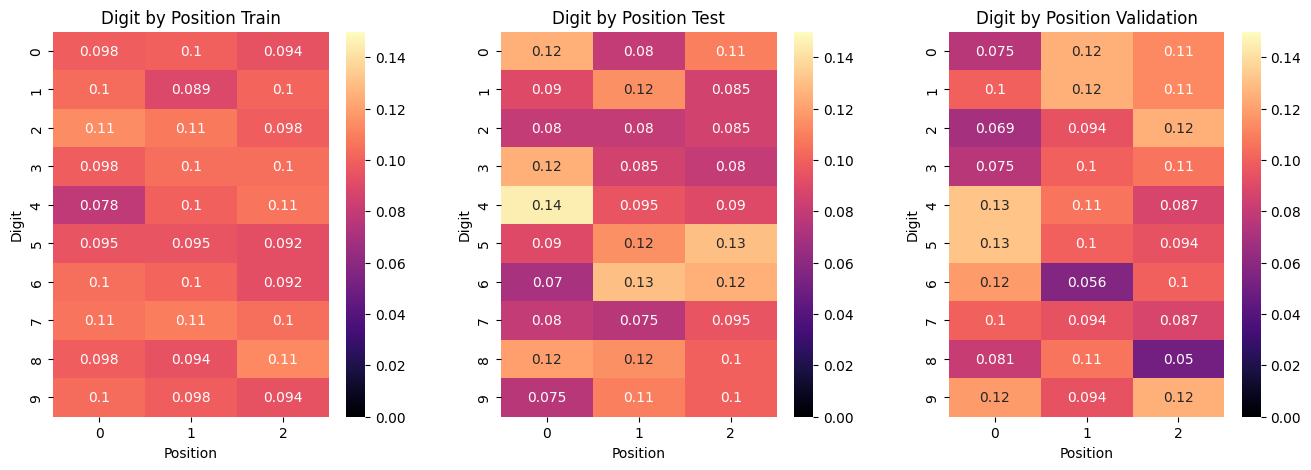
\includegraphics[width=\textwidth, height=5cm,keepaspectratio]{task1/classHeatmap}
    \caption[Heatmap for class distribution in dataset]
    {Heatmap for class distribution in dataset}
    \label{fig:heatmap}
\end{figure}

\begin{figure}[h]
    \centering
    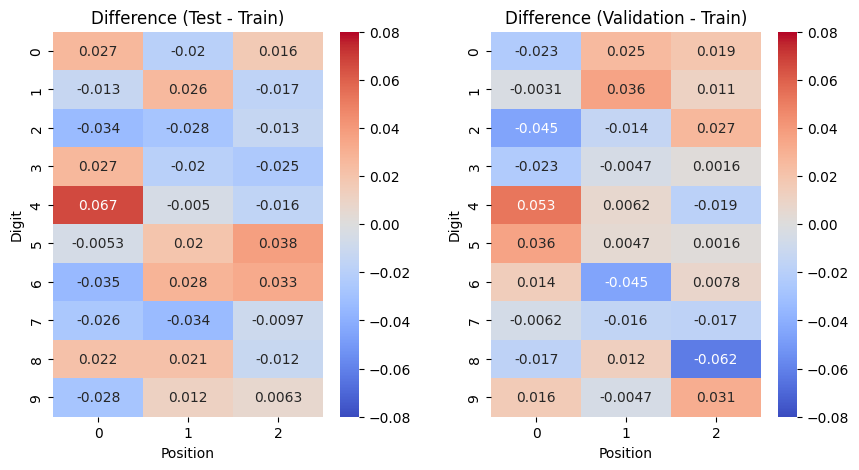
\includegraphics[width=\textwidth, height=5cm,keepaspectratio]{task1/classDifferenceHeatmap}
    \caption[Heatmap for difference in class distribution across dataset]
    {Heatmap for difference in class distribution across dataset}
    \label{fig:digitHeatmap}
\end{figure}

The additional heatmaps in \autoref{fig:digitHeatmap} display the difference between the test and validation sets against the train datasets, designed to highlight any gaps in training. Any digits marked with a positive difference (marked with a red shade) may perform worse in the validation and training evaluations. Digit four in position 1 appears to contain the most positive difference relative to the training set.